\myheading{Multiplication and division using addition and subtraction}

It is possible to use addition instead of multiplication, using the following rule:

\begin{equation} \label{eq:1}
\log_{base} (ab) = \log_{base} (a) + \log_{base}(b)
\end{equation}

\dots while base can be any number.

It's like summing number of zeroes of two numbers. Let's say, you need to multiply 100 by 1000. Just sum number of their zeroes (2 and 3).
The result if the number with 5 zeroes. It's the same as $\log_{10} (100) + \log_{10} (1000) = \log_{10} (100000)$.

Division can be replaced with subtraction in the very same way.

\leveldown{}

\myheading{Logarithmic slide rule}

Here is very typical slide rule\footnote{I took screenshots at \url{http://museum.syssrc.com/static/sliderule.html}}.
It has many scales, but take a look on C and D scales, they are the same:

\begin{figure}[H]
\centering
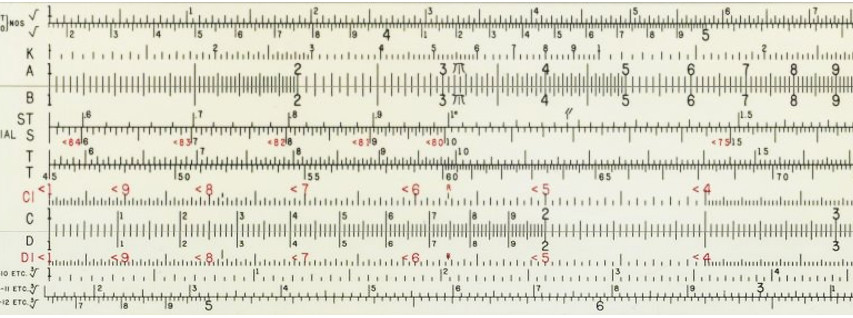
\includegraphics[scale=0.66]{log/sliderule1.jpg}
\caption{Initial state of slide rule}
\end{figure}

Now shift the core of rule so C scale at 1 will point to 1.2 at D scale:

\begin{figure}[H]
\centering
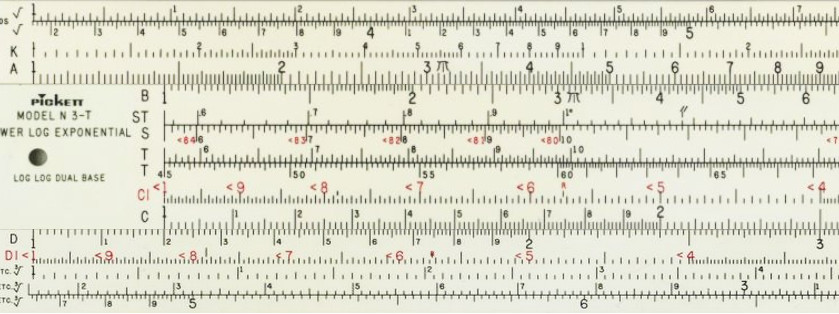
\includegraphics[scale=0.66]{log/sliderule2.jpg}
\caption{C scale shifted}
\end{figure}

% TODO дорисовать стрелки как в https://commons.wikimedia.org/wiki/File:Slide_rule_example2_with_labels.svg?uselang=ru

Find 2 at C scale and find corresponding value at D scale (which is 2.4).
Indeed, $1.2 \cdot 2 = 2.4$.
It works because by sliding scales we actually add distance between 1 and 1.2 (at any scale) to the distance between 1 and 2 (at any scale).
But since these scales logarithmic, addition of logarithmic values is the same as multiplication.

Values on scales can be interpreted as values of other order of magnitude.
We can say that 1 at C scale is actually point to 12 at D scale.
Find 1.8 at D scale (which is 18 now), it points somewhere between 21 and 22.
It's close: $12 \cdot 18 = 216$.

It works because of equation \ref{eq:1}.

Here is another example from Wikipedia:

\begin{figure}[H]
\centering
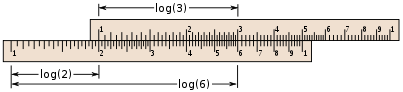
\includegraphics[scale=0.66]{log/403px-Slide_rule_example2_with_labels.png}
\caption{Example from Wikipedia}
\end{figure}

\myheading{Logarithmic tables}

As we can see, the precision of logarithmic slide rule is up to 1 or 2 decimal digits after point.
Using precomputed logarithmic tables, it's possible to calculate product of two numbers with a precision up to $\approx 4$ digits.

First, find common (base of 10) logarithms of each number using logarithmic table:

\begin{figure}[H]
\centering
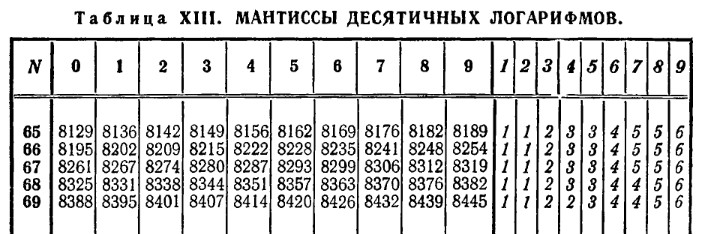
\includegraphics[scale=0.66]{log/bradis1.jpg}
\caption{Logarithmic tables}
\end{figure}

Then add these numbers. Find the number you got in table of powers of 10 ($10^{x}$, also called ``anti-log table''):

\begin{figure}[H]
\centering
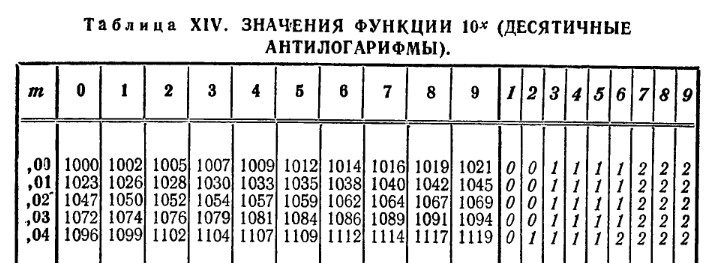
\includegraphics[scale=0.66]{log/bradis2.jpg}
\caption{Antilog tables}
\end{figure}

% TODO CRC book! спросить у него? http://www.mathtable.com/smtf/

Resulting number is a product.
The whole process may be faster than to multiply using long multiplication method using paper-n-pencil taught in schools.

Screenshots I took from the Bradis' book, once popular in USSR.
Another well-known book in western world with logarithmic and other tables is 
Daniel Zwillinger - CRC Standard Mathematical Tables and Formulae 
(up to 30th edition, the logarithmic tables are dropped after).

\myheading{Working with very small and very large numbers}

It's hard to believe, but the rule used on logarithmic slide rule for multiplication is still used sometimes in software code.
It's a problem to work with very small (denormalized) numbers
\footnote{Denormalized numbers in double-precision floating point format are numbers between $\approx 10^{324}$ and $\approx 10^{308}$} encoded in IEEE 754 standard. 

Here is my attempt to calculate $\frac{1.234 \times 10^{-300} \cdot 2.345678901234 \times 10^{-24}}{3.456789 \times 10^{-50}}$:

\begin{lstlisting}[caption=C code]
#include <stdio.h>
#include <math.h>

int main()
{
	double a=1.234e-300;
	double b=2.345678901234e-24;
	double c=3.456789e-50;
	printf ("%.30e\n", a*b/c);
};
\end{lstlisting}

The output is $1.429261797122261460966983388190 \times 10^{-274}$, which is incorrect.
When using debugger, we can see that the multiplication operation raises \textit{inexact exception} and \textit{underflow exception} in FPU.
The division operation also raises \textit{inexact exception}.

Let's check in Wolfram Mathematica:

\begin{lstlisting}[caption=Wolfram Mathematica]
In[]:= a = 1.234*10^(-300);

In[]:= b = 2.345678901234*10^(-24);

In[]:= c = 3.456789*10^(-50);

In[]:= a*b/c
Out[]= 8.37357*10^-275
\end{lstlisting}

The underflow exception raised in my C program because result of multiplication is in fact 
$2.894567764122756*10^{-324}$, which is even smaller than smallest denormalized number FPU can work with.

Let's rework our example to compute it all using natural logarithms 
(\texttt{exp(x)} is a C standard function, which computes $e^x$ and \texttt{log(x)} here is $\log_e(x)$ (or $ln(x)$)):

\begin{lstlisting}[caption=C code]
#include <stdio.h>
#include <math.h>

int main()
{
	double a=1.234e-300;
	double b=2.345678901234e-24;
	double c=3.456789e-50;
	printf ("%.30e\n", exp(log(a)+log(b)-log(c)));
};
\end{lstlisting}

Now the output is $8.373573753338710216281125792150 \times 10^{-275}$, same as Mathematica reported.

The same problem with very large numbers.

\begin{lstlisting}[caption=C code]
#include <stdio.h>
#include <math.h>

int main()
{
	double a=1.234e+300;
	double b=2.345678901234e+24;
	double c=3.456789e+50;
	printf ("%.30e\n", a*b/c);
};
\end{lstlisting}

When this program running, its result is ``inf'', meaning $\infty$, i.e., overflow occurred.
When using debugger, we can see than the multiplication operation raises \textit{inexact exception} plus \textit{overflow exception}.
The correct value in Wolfram Mathematica is...

\begin{lstlisting}[caption=Wolfram Mathematica]
In[]:= a = 1.234*10^300;

In[]:= b = 2.345678901234*10^24;

In[]:= c = 3.456789*10^50;

In[]:= a*b/c
Out[]= 8.37357*10^273
\end{lstlisting}

Let's rewrite our C example:

\begin{lstlisting}[caption=C code]
int main()
{
	double a=1.234e+300;
	double b=2.345678901234e+24;
	double c=3.456789e+50;
	printf ("%.30e\n", exp(log(a)+log(b)-log(c)));
};
\end{lstlisting}

Now the program reports $8.373573753337712538419923350878 \times 10^{273}$, which is correct value.

The way of representing all numbers as their logarithms called ``logarithmic number system''
\footnote{\url{https://en.wikipedia.org/wiki/Logarithmic_number_system}}.
It allows to work with numbers orders of magnitude lower than FPU can handle.

So why all computations are not performed using logarithms, if it's so good?
It's better only for very small or very large numbers.
Working with small and medium numbers, precision of its logarithmic versions will be much more important and harder to control.

Also, finding logarithm of a number with the following exponentiation are operations may be slower than multiplication itself.

\subsection{IEEE 754: adding and subtracting exponents}

IEEE 754 floating point number consists of sign, significand and exponent.
Internally, its simplified representation is:

\begin{equation}
(-1) \cdot sign \cdot significand \times 2^{exponent}
\end{equation}

Given that, the FPU may process significands and exponents separately during multiplication, 
but when it processes exponents of two numbers, they are just summed up.
For example:

\begin{equation}
significand_{1} \times 2^{10} \cdot significand_{2} \times 2^{50} = significand_{3} \times 2^{60}
\end{equation}

\dots precise values of significands are omitted, but we can be sure, if the first number has exponent of $10$, the second has $50$,
the exponent of the resulting number will be $\approx 60$.

Conversely, during division, exponent of divisor is subtracted from the exponent of the dividend.

\begin{equation}
\frac{significand_{1} \times 2^{10}}{significand_{2} \times 2^{50}} = significand_{3} \times 2^{-40}
\end{equation}

I don't have access to Intel or AMD FPU internals, but I can peek into OpenWatcom FPU emulator libraries
\footnote{It was a time in 1980s and 1990s, when FPU was expensive and it could be bought separately 
in form of additional chip and added to x86 computer.
And if you had run a program which uses FPU on the computer where it's missing, FPU emulating library might be an option.
Much slower, but better than nothing.}.

Here is summing of exponents during multiplication:\\
\url{https://github.com/open-watcom/open-watcom-v2/blob/86dbaf24bf7f6a5c270f5a6a50925f468d8d292b/bld/fpuemu/386/asm/fldm386.asm\#L212}.\\
And here is subtracting of exponents during division:\\
\url{https://github.com/open-watcom/open-watcom-v2/blob/e649f6ed488eeebbc7ba9aeed8193d893288d398/bld/fpuemu/386/asm/fldd386.asm\#L237}.

Here is also multiplication function from FPU emulator in Linux kernel:
\url{https://github.com/torvalds/linux/blob/da957e111bb0c189a4a3bf8a00caaecb59ed94ca/arch/x86/math-emu/reg_u_mul.S\#L93}.

%\subsection{Check, if the product will overflow}

% НЕТ

%Using logarithmic versions of two numbers, it is easy to check if the product of them will overflow in current environment (32-bit or 64-bit CPU registers).
%Perhaps, programming languages with dynamic typing (like LISP, Python, Ruby, BASIC, etc) can check, 
%if the current number must be switched to bignum (if the result is too big to fit in the CPU register) or not.

\levelup{}

